\documentclass[a4j]{jarticle}
\title{計算物理学レポート3}
\author{35-196004 天野智仁}
\date{}
\usepackage{listings}	% required for `\lstlisting' (yatex added)
\usepackage[dvipdfmx]{graphicx}	% required for `\includegraphics' (yatex added)
\usepackage{amsmath}	% required for `\align*' (yatex added)
\begin{document}

\section{スピン軌道相互作用を無視したFeの計算}
スピン軌道相互作用を無視したFeの計算は,Wannier90のtutorial example08に置いて示されている.ここで用いられているpseudopotentialはFe.jry.pbe.UPFであり,functionalの形はPBE,pseudopotentialの種類はFull RelativistycでかつUltraSoftである.またvalence bandとして考慮しているのは3D,4S,4Pである.

結果として得られたスピン偏極を含むDOSが下図\ref{120041_4Jul19}である.ただしエネルギーのゼロ点をフェルミレベルに合わせてある.
\begin{figure}[htb]
\centering
 \includegraphics[width=10cm,angle=270]{dos.eps}
\caption{LS相互作用を含まないFeのDOS}
\label{120041_4Jul19}
\end{figure}

系全体の磁化はボーア磁子$\mu_B$及びスピン偏極した電子数$n$を用いて
\begin{align*}
 M&=\mu_B\left(n_{up}-n_{dn}\right) \\
&=\mu_B\left(\int^{E_F}dED_{up}-\int^{E_F}dED_{dn}\right) \\
\end{align*}
となる.これを得られたDOSから計算すると,
\begin{align*}
 Nup&= 5.73278 \\
 Ndn&=10.18045 \\
 Ndn-Nup=4.44767
\end{align*}
となるから従って
\begin{align*}
 M&=5.788\times 10^{-5}\times 4.44767 \\
  &=2.574\times 10^{-4}\mathrm{eV/T}
\end{align*}
を得る.以上から一原子あたりの磁化,磁気モーメントは
\begin{align*}
 \mu&=\frac{M}{2}=2.224\times \mu_B \\
    &=1.287\times 10^{-4}\mathrm{eV/T}
\end{align*}
となる.これは実験で得られる値$2.219\mu_B$と近くなっている.

一方でバンド図は図\ref{121206_4Jul19}となる.
\begin{figure}[htb]
\centering
 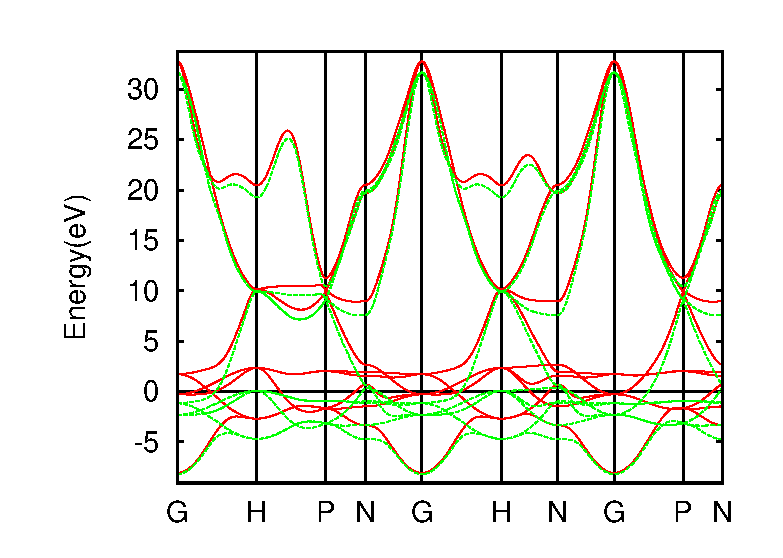
\includegraphics[width=10cm]{band.eps}
\caption{LS相互作用を含まないFeのBAND}
\label{121206_4Jul19}
\end{figure}
赤がスピンup,緑がスピンdnのバンドを表している.これを見てもスピンによってエネルギーが分裂している様子を見ることができる.

\section{スピン軌道相互作用を考えたFeの計算}
次に,スピン軌道相互作用を考えた計算は,example17において示されている.スピン軌道相互作用を考える場合,これによってエネルギー準位の縮退が解けることが期待されるのでそれを調べよう.

まず,QEでスピン軌道相互作用を考慮した計算を行うためには,まずはpseudopotentialとして,scalar relativisticなものではなく,full relativisticなものを使わなければならない.前節で指摘したように今回の計算で使っているのはfull relativisticなものなのでこの点については問題ない.次に,input fileに次の設定を加える必要がある
\begin{lstlisting}
 &system
    lspinorb=.true.
    noncolin=.true.
\end{lstlisting}
また,diagonalizationはexampleのデフォルト'cg'では収束せず,'david'に変更する必要があった.

こうして計算して得られたBAND図は図\ref{122604_4Jul19}である.
\begin{figure}[htb]
\centering
 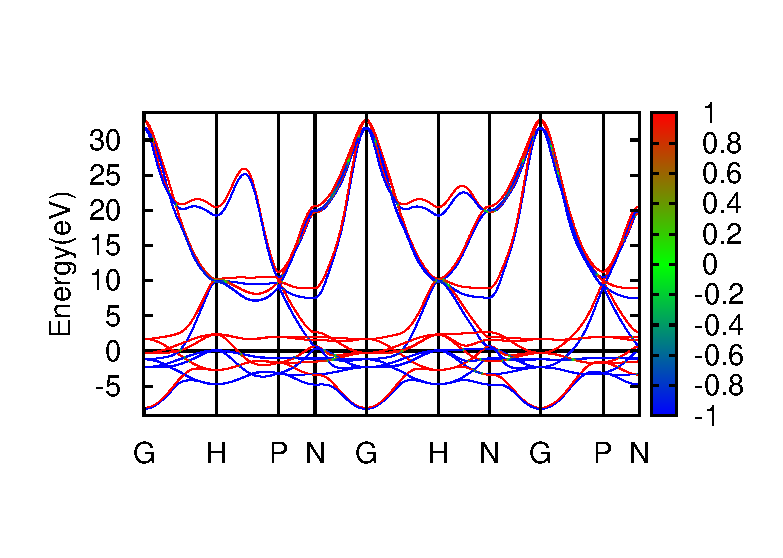
\includegraphics[width=10cm]{bandLS.eps}
\caption{LS相互作用を含むFeのBAND}
\label{122604_4Jul19}
\end{figure}




\section{Berry 位相の計算}
K点メッシュは$1000$点,軌道としてはsp3d2,dxy,dxz,dyzを考えている.こうして得られたberry位相は図のようになった.
\begin{figure}[htb]
 \centering
\includegraphics[width=10cm]{Fe-bands+curv_y.pdf}
\caption{ベリー位相の$y$成分}
\end{figure}

\begin{figure}[htb]
 \centering
\includegraphics[width=10cm]{Fe-bands+curv_z.pdf}
\caption{ベリー位相の$z$成分}
\end{figure}




\end{document}